\documentclass[a4paper,10pt]{article} % Default font size and paper size

\usepackage{xunicode,xltxtra,url,parskip} % Formatting packages

\usepackage[usenames,dvipsnames]{xcolor} % Required for specifying custom colors

\usepackage[big]{layaureo} % Margin formatting of the A4 page, an alternative to layaureo can be \usepackage{fullpage}
% To reduce the height of the top margin uncomment: \addtolength{\voffset}{-1.3cm}

\usepackage{placeins}

\usepackage{hyperref} % Required for adding links	and customizing them
\definecolor{linkcolour}{rgb}{0,0.2,0.6} % Link color
\hypersetup{colorlinks,breaklinks,urlcolor=linkcolour,linkcolor=linkcolour} % Set link colors throughout the document

% For adding publication lists
\PassOptionsToPackage{%
backend=biber,
bibencoding=utf8,
language=auto,
style=authoryear,
maxbibnames=10
}{biblatex}
\usepackage{biblatex}
\addbibresource{references.bib}

\title{Paragraphs for Review Paper}
\author{Alec Hoyland}


\begin{document}

\maketitle

\section{Model selection for Figs. 2 and 3}

Each network model is treated as a directed graph.
In neuronal models, each node is a neuron and each edge is a synaptic connection.
In artificial neural network models, nodes receive input from other nodes modulated by weight parameters.
Intrinsic parameters are any parameters specific to nodes and not connections between them.
Synaptic parameters are any parameters specific to connections (edges) and not nodes.

\subsection{Neuroscience models}

Neuroscience models were selected by working from models classifed as ``Realistic Networks'' on Model DB.

Neuronal morphology is often discretized into compartments for computational purposes.
Therefore, one neuron can be modeled as one or more compartments.
Each compartment contains Hodgkin-Huxley-type conductances and other cellular mechanisms,
such as calcium buffering.
Each compartment contains a number of parameters proportional to the number of conductances and mechanisms.
Most conductances contribute 1 intrinsic parameter per conductance (the maximal conductance)
and most calcium buffering mechanisms contribute 2 intrinsic parameters (buffering rate and steady-state concentration).
Compartments also have a shape, which contributes 1-2 spatial parameters,
as well as a specific membrane capacitance, which contributes 1 intrinsic parameter.
All of these parameters can vary in neuronal models, though they need not necessarily.
Injected current and choice of initial conditions were not considered.

Some parameters are considered ``environmental'', i.e. they apply to the entire model
and are invariant across compartments and neurons due to physical constraints.
Examples of these intrinsic parameters include temperature and ion reversal potentials.
These parameters were only counted once each.

Generally, there is 1 synaptic parameter per synapse, corresponding to the synaptic strength.

\subsection{Computer science models}

Some of the most influential models in recent years were considered.

For most models, there were 3 intrinsic parameters per node,
corresponding to the choice of activation function parameters.

The strength of each connection between nodes is determined by a weight parameter,
so there is 1 synaptic parameter per connection.
Bias parameters were also factored in as synaptic parameters.

\section{Exploring parameter spaces}

Biophysically realistic neuronal and network models can be high-dimensional, with many tunable parameters,
leading to complications in characterizing the model.
Models that incorporate more neurons or neuronal complexity exponentially increase the size of the parameter space.
Due to the size of the parameter space, hand-tuning parameters is a difficult prospect.
For instance, to characterize a parameter space of 6 dimensions at 10 values per parameter requires $6^{10}$ simulations.
While there exists simulation software which can integrate models very quickly
\parencite{gorur-shandilyaXolotlIntuitiveApproachable2018, bretteSimulationNetworksSpiking2007},
characterizing an entire parameter space quickly becomes unfeasible.

One possible strategy to characterize the space is to simulate at selected points in the parameter hypercube
and build a searchable database. \cite{prinzAlternativeHandtuningConductancebased2003}
varied 8 maximal conductance parameters in a lobster stomatogastric neuron model
and produced a database of about 1.7 million models.
This process took over a month of simulations on a high-performance computing cluster.
While processor speed has increased threefold since this publication,
characterizing a parameter space by random or grid-spaced parameter sweeps is computationally infeasible.

More recently, parameter optimization algorithms have been used to find model parameters that satisfy some search criteria
\parencite{hoylandDifferentialResponsesNeuromodulation2018, gorur-shandilyaXolotlIntuitiveApproachable2018, alonsoVisualizationCurrentsNeural2019}.
Optimization algorithms minimize an objective function, which accepts the parameters as input,
and outputs a positive value corresponding to the fitness of the model.
The choice of objective function is arbitrary but should reflect the desired neurocomputational properties of the model.
Parameter optimization algorithms adjust the parameters of the model to find a local minimum of the objective function
and therefore find parameters of the model which produce the desired activity \parencite{bangaOptimizationComputationalSystems2008}.
This has the advantage of arriving at desired model activity without having to search the entire parameter space.
Parameter optimization avoids the disadvantages of wholesale parameter sweeps,
however it relies on an arbitrary objective function
and requires many integrations of the network model.

A new technique, simulation-based inference expedites the search process
by developing a statistical inference model relating parameters to anticipated model outputs.
Statistical inference uses the likelihood function $p(x | \theta)$ to quantify
how well the parameters $\theta$ satisfy the constraints of the data $x$.
For mechanistic models of neuron and network function, such as conductance-based models in the Hodgkin-Huxley formalism
\parencite{hodgkinQuantitativeDescriptionMembrane1952},
likelihood functions are unavailable.
New advantages in likelihood-free statistical inference have led to
new parameter estimation methods applicable to neuron and network models \parencite{cranmerFrontierSimulationbasedInference2019}.
Simulations conditioned on parameters sampled from within the entire parameter space
are used to train an artificial neural network which outputs a posterior distribution over all parameters
\parencite{goncalvesTrainingDeepNeural2019, lueckmannFlexibleStatisticalInference2017}.
This method requires generating a large amount of synthetic data before training the neural network
but obviates the need for computationally expensive simulations when estimating parameters.
This method also returns the full posterior distribution over all parameters,
which permits identifying trajectories through parameter space where network activity is preserved.

\section{Network degeneracy}

In the context of biological systems, degeneracy refers to a redundancy in function,
where multiple elements that are structurally or parametrically different can perform the same function
or produce similar output \parencite{edelmanDegeneracyComplexityBiological2001a, tononiMeasuresDegeneracyRedundancy1999}.
Models of neurons and networks are frequently degenerate with many parameter sets yielding similar simulated activity
\parencite{prinzAlternativeHandtuningConductancebased2003, prinzSimilarNetworkActivity2004, achardComplexParameterLandscape2006}.
Taking parameter averages or assuming one ``optimal'' solution is insufficient
\parencite{loebOptimalIsnGood2012, golowaschFailureAveragingConstruction2002}.
Experimental recordings reveal underlying animal-to-animal variability
that converges to stable, rhythmic motor patterns
\parencite{bucherAnimaltoanimalVariabilityMotor2005, hamoodAnimaltoanimalVariabilityNeuromodulation2014,
roffmanAnimaltoanimalVariabilityConnection2012, marderVariabilityCompensationModulation2011}.

Degeneracy is a mechanism common to neural systems
\parencite{whitacreDegeneracyDesignPrinciple2010, stellingRobustnessCellularFunctions2004,
goldmanGlobalStructureRobustness2001, tononiMeasuresDegeneracyRedundancy1999}.
\cite{rathourDegeneracyHippocampalPhysiology2019} provide an excellent review
of biological degeneracy at all scales in the hippocampus.
Degeneracy provides flexibility in achieving conjoint goals of remaining sensitive
to endogenous signals yet robust to external perturbation
\parencite{marderNeuromodulationCircuitsVariable2014, olearyCorrelationsIonChannel2013}.
A motor circuit governed by a central pattern generator must maintain activity
over long periods while remaining responsive to endogenous neuromodulation
\parencite{marderHowCanMotor2015}.
Similarly, the hippocampus must be able to encode new data while preserving existing information
\parencite{mauSameHippocampalCA12018, piatkevichPopulationImagingNeural2019}.
The mechanisms by which degeneracy engenders robustness to perturbation
have been extensively studied in small circuit neuroscience
\parencite{marderRobustCircuitRhythms2015, marderHowCanMotor2015, marderVariabilityCompensationModulation2011}.
For instance, the crustacean stomatogastric ganglion preserves rhythmicity
during temperature fluctuations of up to 15 degrees Celsius
\parencite{tangRobustnessRhythmicCircuit2012, rinbergEffectsTemperatureStability2013,
soofiPhaseMaintenanceRhythmic2014, marderRobustCircuitRhythms2015,
haddadCircuitRobustnessTemperature2017, tangPreciseTemperatureCompensation2010}.
Temperature compensation has also been observed in leeches
\parencite{arbasRateModificationHeartbeat1984}
and grasshoppers \parencite{roemschiedCellintrinsicMechanismsTemperature2014}.
Modeling studies show that many parameter sets maintain rhythmic activity under temperature increases
\parencite{caplanManyParameterSets2014, alonsoVisualizationCurrentsNeural2019}.

Degeneracy in parameter space can be visualized using pairwise scatter plots.
Methods of dimensionality reduction distort the parameter space,
so it is better to examine pairwise ``snapshots'' of parameter space
than to compress a high-dimensional space onto a 2-dimensional manifold.
Figure \ref{fig:correlationsab} visualizes the space of conductance parameters
of the AB-PD neuron in a model of the pyloric network in the crustacean stomatogastric ganglion
\parencite{hoylandDifferentialResponsesNeuromodulation2018, prinzSimilarNetworkActivity2004}.
Each black dot corresponds to a parameter set that produces normal pyloric activity in the simulated model.
Each red dot corresponds to a parameter set that responds appropriately to endogenous modulation
by red pigment concentrating hormone
\parencite{swensenModulatorsConvergentCellular2001, nusbaumRolesCotransmissionNeural2001,
swensenMultiplePeptidesConverge2000}.
The parameter space is very diffuse but significant correlations between parameters still exist
(bolded axes).
Maintaing these relationships is part of homeostatic control at both the protein and transcriptional level
\parencite{schulzVariableChannelExpression2006a, olearyCorrelationsIonChannel2013,
marderNeuromodulationCircuitsVariable2014}.

\begin{figure}
	\centering
	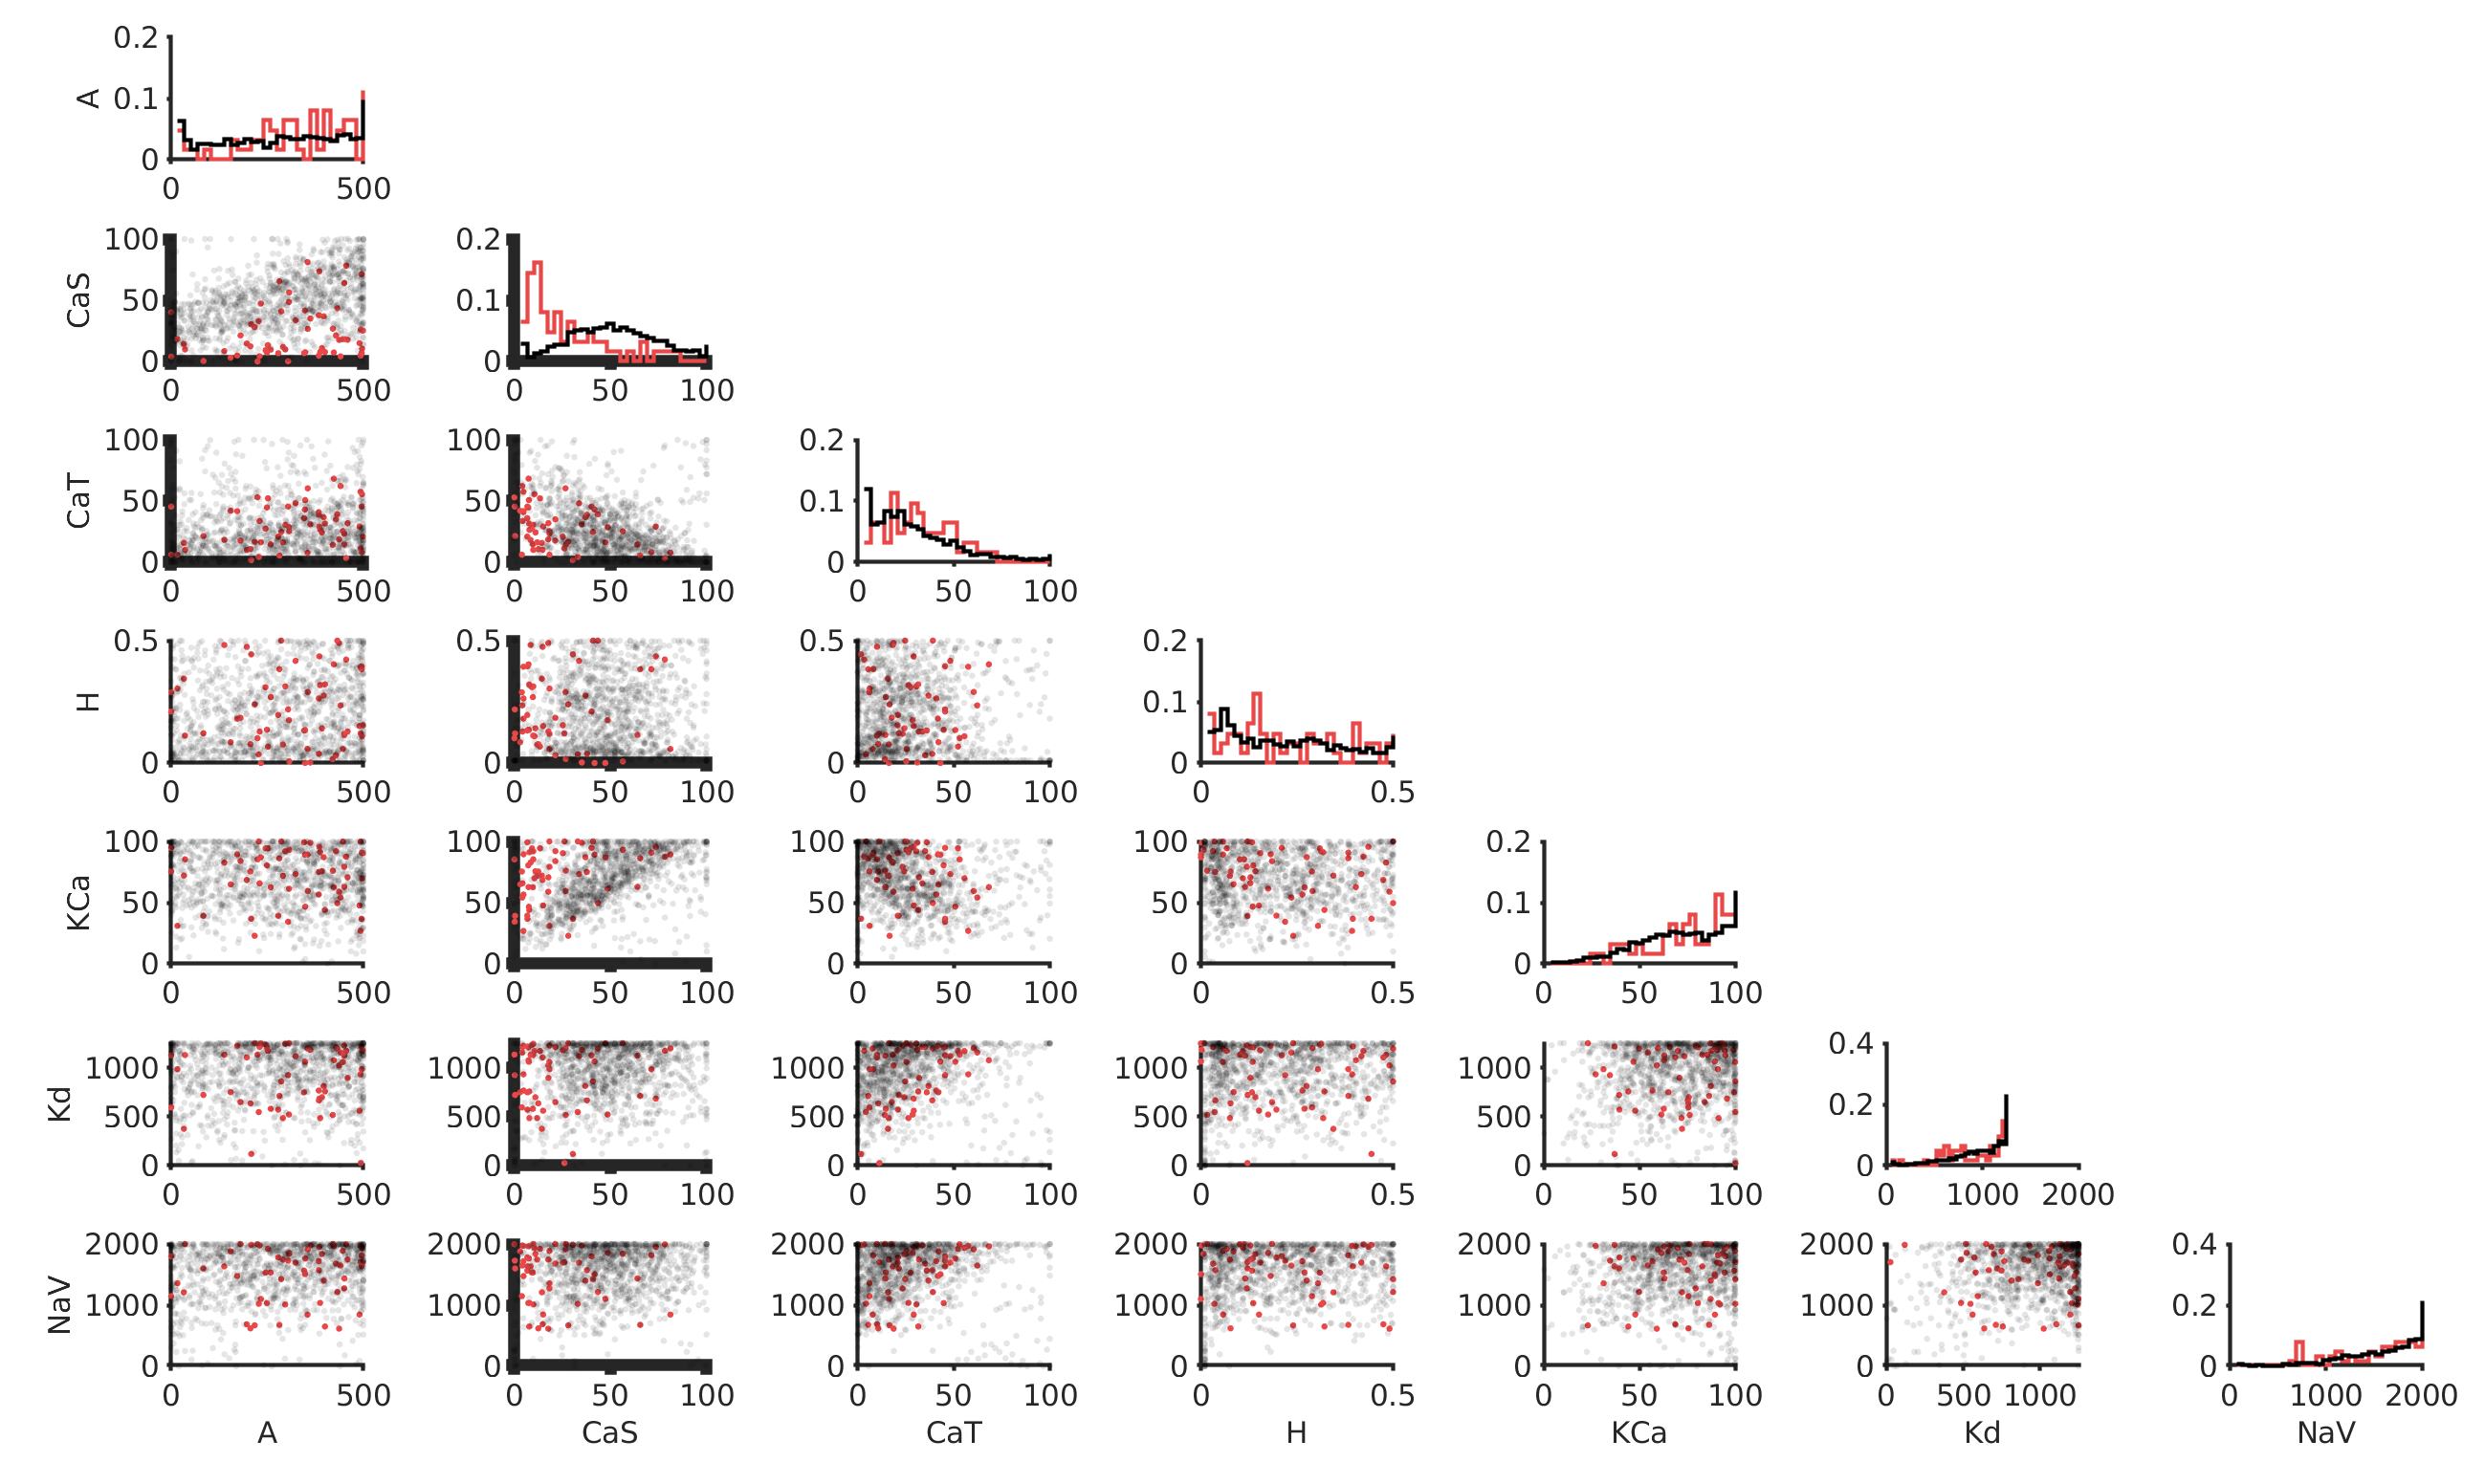
\includegraphics[width=0.9\linewidth]{gfx/correlations_AB.eps}
	\caption{Cross-correlation in {AB}-{PD} maximal conductances from network models. Maximal conductances from control networks (black, $n=1,148$), which are pyloric in non-modulated conditions, and optimized models (red, $n=82$), which are non-pyloric in non-modulated conditions and pyloric under modulation onto {AB}-{PD} and {LP}, are plotted against each other. Plots on the diagonal are histograms of maximal conductance. normalized to population size in each case. \textbf{Bold} axes indicate significant correlation (Kolmogorov-Smirnov 2-tailed 2-D test, $p<0.05$). All conductances are in $\mu\mathrm{S/mm^2}.$}
	\label{fig:correlationsab}
\end{figure}

\FloatBarrier

In linear algebra contexts, degeneracy refers to matrices of less than full rank.
The vector space spanned by a degenerate matrix is smaller in dimensionality
than that of a higher rank matrix of the same size.
Artificial neural networks with degenerate weight matrices train poorly
\parencite{orhanSkipConnectionsEliminate2018a, penningtonResurrectingSigmoidDeep2017, saxeExactSolutionsNonlinear2014}.
While degeneracy in parameters or function \textit{within the same model}
reduces the degrees of freedom and should be avoided,
artificial neural networks are just as susceptible to the biological definition of degeneracy
as true biological networks and models thereof.
Two neural networks initialized randomly and trained on the same dataset
may perform equivalently in metrics such as accuracy and perplexity
but may have entirely different underlying parameters.
This phenomenon is not well-studied in the computer science literature;
instead, neural networks are frequently treated as ``blackboxes''
\parencite{novakSensitivityGeneralizationNeural2018, baiUsingPerturbedSystem2009}.

\section{Exploring degenerate parameter spaces}

Adaptive sampling can be used to efficiently sweep a parameter space.
Instead of sampling along grid spaces, adaptive sampling algorithms
sample more closely when the metric of interest is changing
and sample more slowly when the metric is slowly varying or invariant.
Adaptive sampling algorithms can effectively identify boundaries in parameter space.
In 2 dimensions, Delaunay triangularization can be used to partition a space into searchable regions
which can then be efficiently explored.
Figure \ref{fig:sampling} shows the results of an adaptive sampling algorithm
operating over two parameters of a stomatogastric ganglion neuron model
\parencite{liuModelNeuronActivityDependent1998}.
The burst period of the neuron depends on the slow calcium conductance ($g_{CaS}$)
and the hyperpolarization-activated mixed cation conductance ($g_H$).
The algorithm samples more closely when the absolute value of the gradient of the burst period
with respect to the parameters is high,
in order to efficiently sample regions of interest.

\begin{figure}
  \centering
  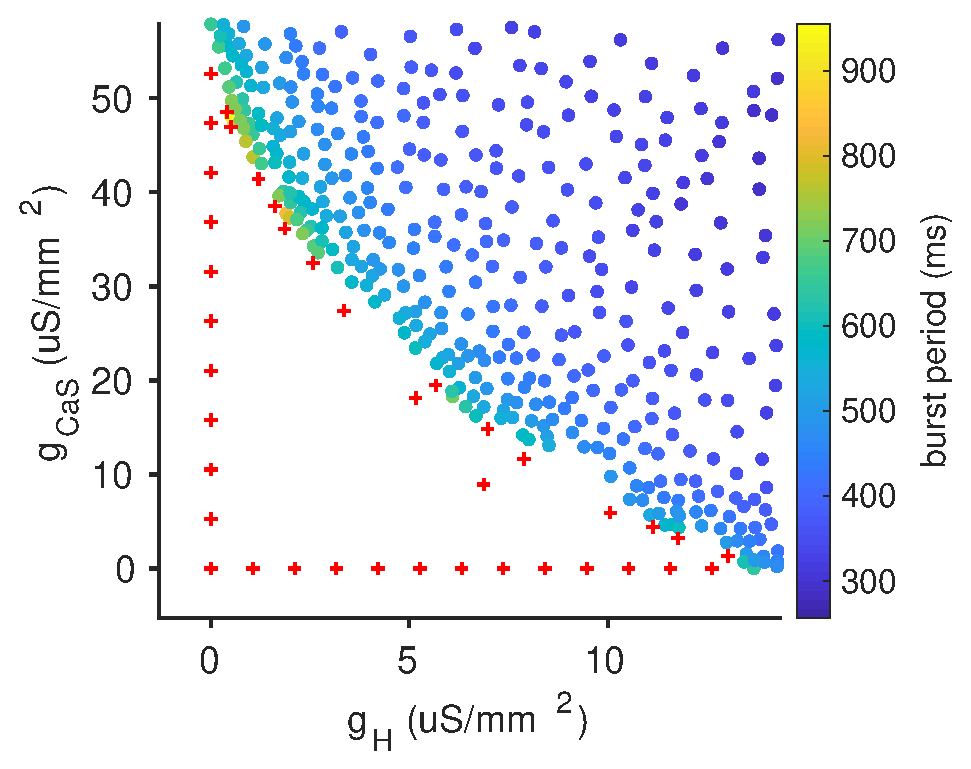
\includegraphics[width=0.6\textwidth]{gfx/demo_adaptive_sampling.eps}
  \caption{Adaptive sampling of two parameters to characterize burst period.
  Red plusses indicate boundaries of the null region (no bursting in the model).
  Dots indicate sampled parameter values. Dots are colored based on observed burst period.
  Dots are clustered where the burst period covaries with the parameters most strongly.}
  \label{fig:sampling}
\end{figure}

\FloatBarrier

Particle swarm performs well on ``pockmarked'' objective function landscapes,
where there are many local minima corresponding to degenerate solutions
\parencite{coventryHierarchicalWinnertakeallParticle2017, hoylandDifferentialResponsesNeuromodulation2018}.
Figure \ref{fig:optimization} shows benchmarks for three optimization algorithms
implemented in the simulation software \textsc{xolotl} \parencite{gorur-shandilyaXolotlIntuitiveApproachable2018}.
An 8-parameter model of a stomatogastric ganglion cell \parencite{prinzAlternativeHandtuningConductancebased2003}
was optimized for desired burst frequency, mean number of spikes per burst, and duty cycle
using a pattern search algorithm \parencite{hookeDirectSearchSolution1961},
a genetic algorithm \parencite{mitchellIntroductionGeneticAlgorithms2001},
and particle swarm optimization \parencite{kennedyParticleSwarmOptimization1995}.
A cost of 0 means that the model's neurocomputational properties lie within specified ranges
and the objective is met.
Initial parameter values were determined randomly.
Since genetic algorithms and particle swarm are stochastic optimization algorithms,
the optimizations were repeated multiple times with the same initial conditions and parameter values.
Since particle swarm samples many points in parameter space at once
during each step of the optimization process,
the algorithm can find a local minimum corresponding to a degenerate solution very quickly.

\begin{figure}[h]
  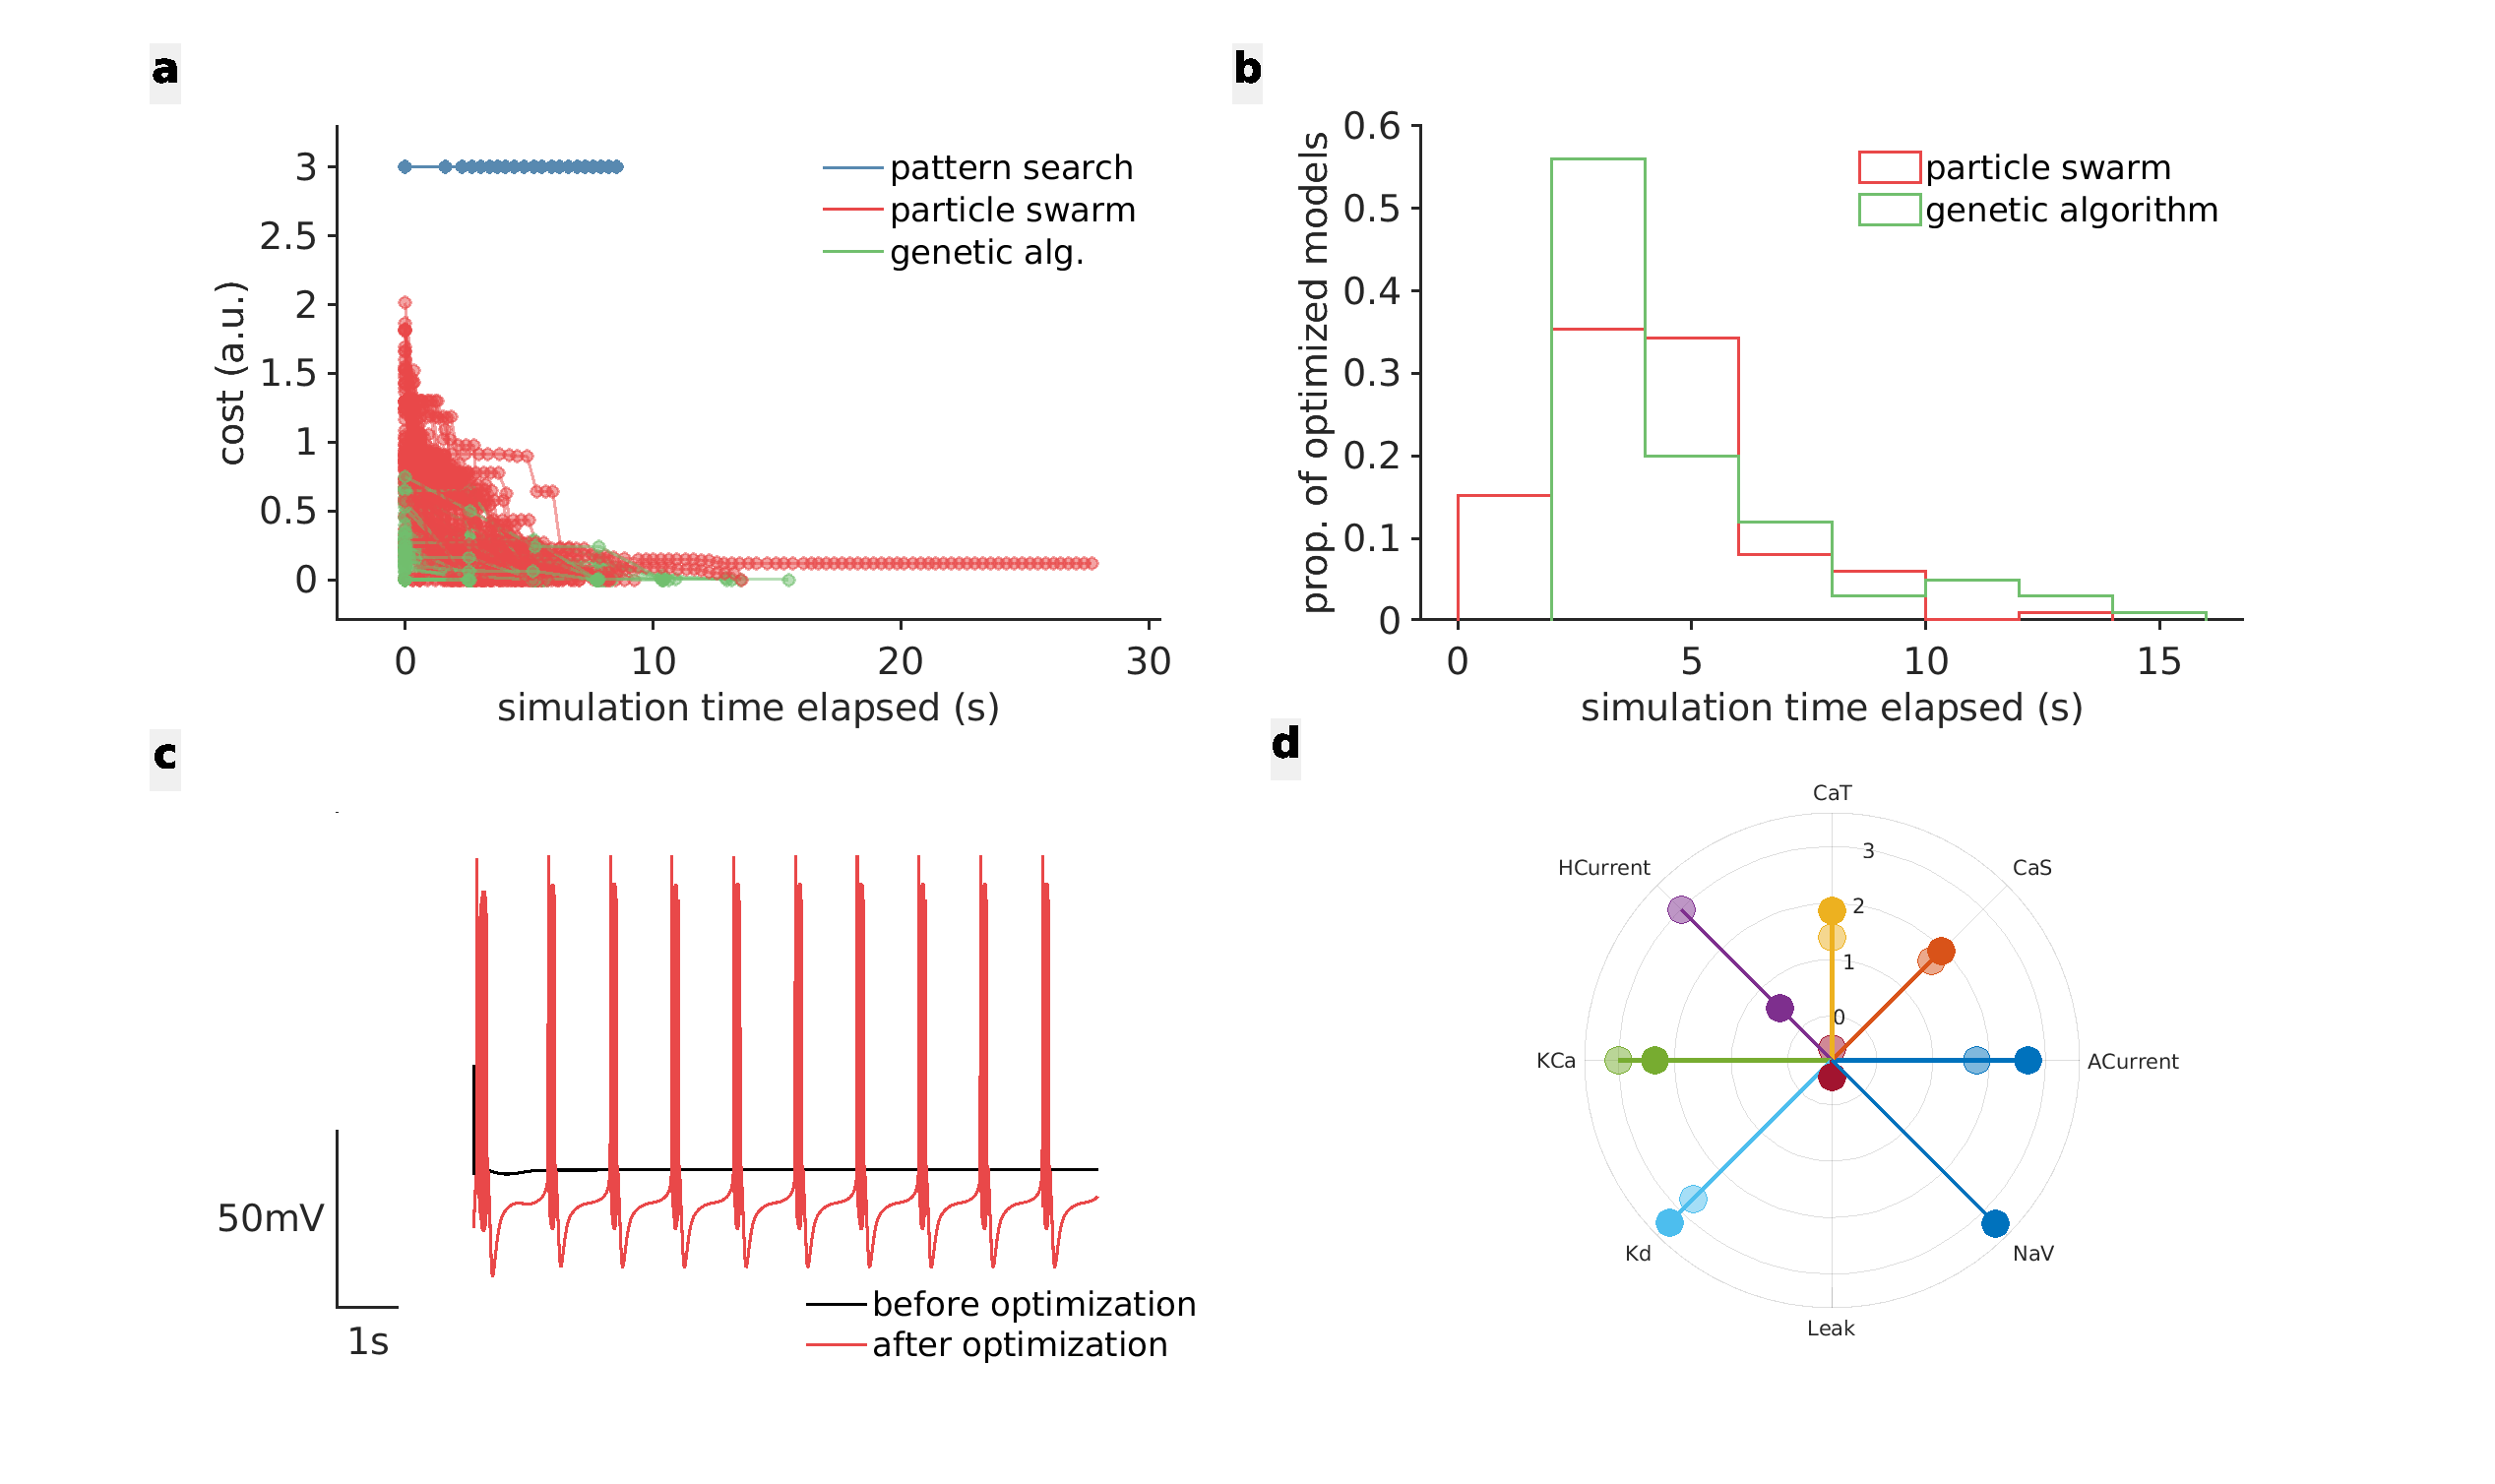
\includegraphics[width=\textwidth]{gfx/figure_param_opt_benchmark.eps}
  \caption{Benchmark of parameter optimization algorithms. (a) Cost over time for the cost func-
  tion measuring burst frequency, mean number of spikes per burst, and duty cycle, as a function of
  real time. A cost of zero indicates a model that satisfies all constraints. Colors indicate different
  algorithms used. Particle swarm and genetic algorithm are stochastic and were simulated 100 times
  each (multiple trajectories plotted). (b) Proportion of models reaching a cost of zero during optimization
  as a function of the optimization time. (c) Waveform of model before optimization (black)
  and waveform after particle swarm optimization with zero cost (red). (d) Depiction of the conductance parameters
  in base-10 logarithmic units for the model before optimization (transparent) and after optimization depicted in (c).}
\label{fig:optimization}
\end{figure}

\FloatBarrier


\printbibliography


\end{document}
